\documentclass[a4paper,10pt]{article}
\usepackage{graphicx}
\usepackage[a4paper, margin=1in]{geometry}
\usepackage{fontawesome} 
\usepackage{color}
\usepackage{titlesec}
\usepackage{enumitem}
\usepackage{pgf-pie} 
\usepackage{hyperref}

% Couleurs
\definecolor{darkblue}{RGB}{25, 25, 112}
\definecolor{gray}{RGB}{105, 105, 105}
\definecolor{lightgray}{RGB}{240, 240, 240}


\titleformat{\section}
{\color{darkblue}\normalfont\Large\bfseries}
{}{0em}{}[\titlerule]

\hypersetup{
    colorlinks=true,
    linkcolor=darkblue, % Couleur des liens
    urlcolor=darkblue, % Couleur des URLs
}


\newcommand{\iconitem}[2]{%
    \ifx&#2&%
        \item[—] #1 
    \else%
        \item[#2] #1 
    \fi%
}

\begin{document}

% Header section with LinkedIn and GitHub links
\begin{center}
    {\Huge \textbf{Bastide Davoux}} \\
    \vspace{0.2cm}
    \textcolor{gray}{Data Manager} \\
    \vspace{0.2cm}
    \vspace{0.5cm}
    \faEnvelope \, \texttt{bastide.60@gmail.com} \quad
    \faPhone \, 06 58 14 63 79 \quad
    \faHome \, 94800 Villejuif, France \\
    \vspace{0.2cm}
    \faLinkedinSquare \, \href{https://www.linkedin.com/in/bastide-davoux-74a17a1b9/}{LinkedIn} \quad
    \faGithub \, \href{https://github.com/bdavoux/Projets}{GitHub} \\
    \vspace{0.5cm}
  \textit{CV codé sur Overleaf en LaTeX. Code source disponible sur \href{https://github.com/bdavoux/Projets}{GitHub}}

    \vspace{0.5cm}
\end{center}

% Professional Summary with text on the left and pie chart on the right
\section*{Profil professionnel}
\begin{minipage}{0.6\textwidth} % Adjust width of text area
    Curieux et autonome, j'occupe actuellement le poste de Data Governance Manager, avec une spécialisation en gestion de la qualité des données. Après avoir acquis une expérience significative en tant que Data Manager, je souhaite explorer de nouvelles opportunités. Je suis prêt à relever de nouveaux défis qui me permettront d'élargir mes compétences et de mettre à profit mon expertise en gestion des données, en automatisation, ainsi qu'en visualisation.
\end{minipage}%
\hfill
\begin{minipage}{0.35\textwidth} % Adjust width of chart area
    \begin{center}
        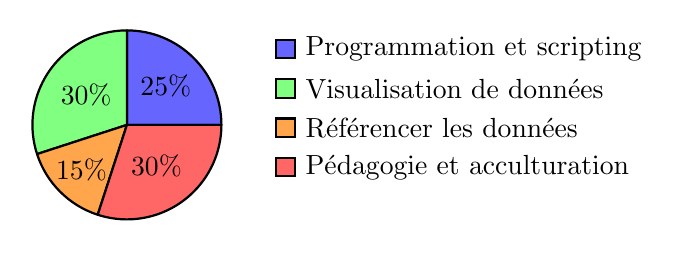
\begin{tikzpicture}[scale=0.4] % Reduces the size of the pie chart by half
            \pie[color={blue!60, green!50, orange!70, red!60}, text=legend]
            {25/Programmation et scripting, 30/Visualisation de données, 15/Référencer les données, 30/Pédagogie et acculturation }
        \end{tikzpicture}
    \end{center}
\end{minipage}





\vspace{0.3cm}

% Skills section with icons
\section*{Compétences techniques}
\begin{itemize}
    \iconitem{\textbf{Langages de programmation} : Python, Java, C, C\#, PHP, JavaScript}{\faCode}
    \iconitem{\textbf{Bases de données} : PostgreSQL, Oracle, AWS, MySql}{\faDatabase}
    \iconitem{\textbf{Outils et plateformes Big Data} : Dataiku, Databricks, Amazon S3, AWS Glue}{\faCloud}
    \iconitem{\textbf{Outils de visualisation} : QlikSense, Metabase, Excel}{\faLineChart}
    \iconitem{\textbf{Automatisation} : Scripts Python, Dataiku (scénarios), VBA, Planificateur de taches}{\faCog}
    \iconitem{\textbf{Systèmes d'exploitation} : Unix, Linux (Ubuntu, Kali), Windows}{\faCogs}
    \iconitem{\textbf{Langages de requête} : SQL, SOQL (SalesForce), Power Query}{\faDatabase}
\end{itemize}

\vspace{0.3cm}

% Professional Experience
\section*{Expérience professionnelle}

\subsection*{Data Governance Manager, Lefebvre-Dalloz - CDI \hfill Depuis 2023}
\begin{itemize}
    \iconitem{Création de scripts (SQL et Python sur Dataiku) pour suivre la qualité des données du FU et identifier les doublons. Le résultat de cet audit est disponible sur un dashboard Metabase.}{\faChevronRight}
    \iconitem{Développement de tableaux de bord sur QlikSense pour permettre aux équipes métiers un suivi des données, en affichant les cibles de qualité.}{\faChevronRight}
    \iconitem{Réalisation de tableaux de bord QlikSense pour suivre la qualité des données (taux de complétude du SIRET, téléphone, etc.) à destination des référents métiers.}{\faChevronRight}
    \iconitem{Automatisation du nettoyage et de la normalisation des données, facilitant l'amélioration continue des processus métier.}{\faChevronRight}
    \iconitem{Collaboration avec les équipes de Data Science pour définir des KPI's.}{\faChevronRight}
    \iconitem{Tenue du dictionnaire de données de l'entreprise et réalisation de lineages sur DataGalaxy}{\faChevronRight}
    \iconitem{Développement d'un script Python pour automatiser la mise à jour du référentiel de cookies.}{\faChevronRight}
\end{itemize}

\vspace{0.3cm}

% Personal Projects
\section*{Projets réalisés}

\subsection*{Application en langage C de gestion d'une entreprise de location de véhicules}
\begin{itemize}
    \iconitem{Développement d'une application complète pour la gestion d'une flotte de véhicules de location.}{\faChevronRight}
\end{itemize}

\subsection*{Applications bancaires pour étudiants (Oracle \& PostgreSQL)}
\begin{itemize}
    \iconitem{Conception de l'architecture de données pour la gestion des prêts étudiants, en utilisant la modélisation MERISE et en assurant les aspects d'administration des bases de données (optimisation, sécurité et sauvegarde).}{\faChevronRight}
    \iconitem{Déploiement des bases de données sur Oracle et PostgreSQL, et mise en place des systèmes pour la gestion des prêts.}{\faChevronRight}
\end{itemize}

\subsection*{Site web pour une entreprise de dératisation (PHP, HTML, CSS, MySQL)}
\begin{itemize}
    \iconitem{Conception et développement d'un site web pour une entreprise de dératisation avec une base de données MySQL pour gérer les commandes clients.}{\faChevronRight}
\end{itemize}

\subsection*{Jeu du Trivial Pursuit en C\#}
\begin{itemize}
    \iconitem{Développement d'une application de jeu Trivial Pursuit en C\# avec gestion des interfaces graphiques et des mécaniques de jeu.}{\faChevronRight}
\end{itemize}

\subsection*{Application Java de gestion de bibliothèque personnelle (Google Books API)}
\begin{itemize}
    \iconitem{Intégration de l'API Google Books pour automatiser l'enregistrement des livres dans la bibliothèque personnelle.}{\faChevronRight}
    \iconitem{Création d'un algorithme performant pour suggérer des lectures à l'utilisateur en fonction des livres enregistrés.}{\faChevronRight}
\end{itemize}

\vspace{0.3cm}

% Education and Certifications
\section*{Formations et Certifications}
\subsection*{Master P.I.S.E (Projets Informatiques et Stratégie d’Entreprise), Université Paris-Cité\hfill{Diplôme obtenu en 2024}}
Objectif: acquérir un solide bagage technique sur
 les systèmes d’information (programmation
 procédurale et objet, bases de données, réseaux,
 web, etc.)
\begin{itemize}
    \iconitem{Programmation : Python, Java, C, PHP, C\#}{}
    \iconitem{Bases de données : SQL, Oracle, PostgreSQL}{}
    \iconitem{Analyse de données, modélisation et gestion des systèmes d’information}{}
\end{itemize}

\subsection*{Certifications}
\begin{itemize}
    \iconitem{Dataiku Core Designer}{\faCertificate}
    \iconitem{Certificat Voltaire (Expression orale/écrite)}{\faCertificate}
\end{itemize}

\vspace{0.3cm}

\end{document}
